%---------------------------------------------------------------------------------------------------------
%---------------------------------------------------------------------------------------------------------
\section{Introduction}

Nous allons dans cette partie voir une m\'ethode de r\'esolution num\'erique d'un probl\`eme simple de
contr\^ole optimal utilisant les conditions n\'ecessaires d'optimalit\'e, c'est-\`a-dire le Principe
du Maximum de Pontryagin (PMP), \cf annexe \ref{chap:pmp_fort}. Cette m\'ethode fait partie des m\'ethodes dites indirectes et s'appelle
la m\'ethode de tir simple.
%Vous pouvez consulter la r\'ef\'erence suivante pour une description
%des diff\'erentes m\'ethodes num\'eriques de r\'esolution de probl\`emes de contr\^ole optimal~: A.~V.~Rao,
%\emph{A survey of numerical methods for optimal control}.

%---------------------------------------------------------------------------------------------------------
%---------------------------------------------------------------------------------------------------------
\section{Pr\'esentation de la m\'ethode de tir simple sur un exemple}

\subsection{Le probl\`eme de contr\^ole optimal}

    Consid\'erons le probl\`eme de contr\^ole optimal suivant.
    \leqnomode
    \begin{equation}
    \tagProblem
        \left\{ 
            \begin{array}{l}
                \displaystyle J(u(\cdot))  \coloneqq \displaystyle \frac{1}{2} \int_0^{t_f} u(t)^2 \, \diff t\longrightarrow \min \\[1.0em]
                \dot{x}(t)  =  \displaystyle -x(t)+u(t), \quad  u(t) \in \R, \quad t \in \intervalleff{0}{t_f} \text{ p.p.},\quad x(0) = x_0, \\[1.0em]
                x(t_f) = x_f,
            \end{array}
        \right. 
        \label{eq:ocpSimple}
    \end{equation}
    \reqnomode
    avec $t_f \coloneqq 1$, $x_0 \coloneqq -1$, $x_f \coloneqq 0$ et $\forall\, t \in\intervalleff{0}{t_f}$, $x(t) \in \R$.
    Notons 
    \[
        H(x,p,p^0,u) \coloneqq p \, (-x+u) + p^0\, \frac{1}{2} u^2,
    \]
    le pseudo-hamiltonien associ\'e au probl\`eme \eqref{eq:ocpSimple}.

\subsection{Application du principe du maximum de Pontryagin}

    D'apr\`es le PMP, si $u(\cdot)$ est une solution optimal de \eqref{eq:ocpSimple} (avec $x(\cdot)$ la trajectoire associ\'ee)
    alors il existe un vecteur adjoint $p(\cdot) \in AC(\intervalleff{0}{t_f},\R)$, un scalaire $p^0 \le 0$, tels que $(p(\cdot),p^0) \ne (0,0)$,
    et tels que les \'equations suivantes sont v\'erifi\'ees pour $t\in\intervalleff{0}{t_f}$ p.p. :
    \begin{equation*}
        \left\{ 
            \begin{array}{ll}
                \dot{x}(t)  & = \phantom{-} \partial_p H[t] = -x(t)+u(t),   \\[0.5em]
                \dot{p}(t)  & = -           \partial_x H[t] = p(t),         \\[0.5em]
                0           & = \phantom{-} \partial_u H[t] = p(t)+p^0 u(t),
            \end{array}
        \right. 
    \end{equation*}
    o\`u $[t] := (x(t),p(t),p^0,u(t))$.
    Il n'y a pas d'anormale car si $p^0=0$ alors $p(\cdot)\equiv0$ ce qui est impossible. Ainsi, on a $p^0 < 0$.
%
    Notons 
    $
        u_s(x,p,p^0) \coloneqq - p/p^0,
    $
    la solution de l'\'equation $0 = \partial_u H(x,p,p^0,u)$ pour $(x,p,p^0)$ fix\'e.
    On peut alors fixer arbitrairement $p^0\ne 0$ car pour tout $\alpha \in \Rsp$, $u_s(x,\alpha p, \alpha p^0) = u_s(x,p,p^0)$ et la trajectoire
    associ\'ee reste inchang\'ee. Fixons $p^0 = -1$ et notons maintenant
    \begin{equation*}
        u_s(x,p) = p
        %\label{eq:controleOCPSimple}
    \end{equation*}
    le contr\^ole optimal. De m\^eme, on notera $H(x,p,u)$ le hamiltonien tel que $p^0= -1$.

\subsection{Probl\`eme aux deux bouts}

L'application du PMP nous m\`ene \`a r\'esoudre le \emph{probl\`eme aux deux bouts} (Two Points Boundary Value Problem) suivant~:
    \leqnomode
    \begin{equation}
    \tagProblem
        \left\{ 
            \begin{array}{ll}
                \dot{x}(t)  & = -x(t) + u_s(x(t),p(t)) = -x(t)+p(t),              \\[0.5em]
                \dot{p}(t)  & = \phantom{-}p(t),                                    \\[0.5em]
                x(0)        & = x_0, \quad x(t_f) = x_f.
            \end{array}
        \right. 
        \label{eq:bvpSimple}
    \end{equation}
    \reqnomode
    L'inconnue de ce probl\`eme aux deux bouts est le vecteur adjoint initial $p(0)$.
    En effet si l'on fixe $p_0 \coloneqq p(0)$ alors d'apr\`es le th\'eor\`eme de Cauchy--Lipschitz, il existe une unique solution maximale
    $z(\cdot, x_0, p_0)\coloneqq(x(\cdot, x_0, p_0),p(\cdot, x_0, p_0))$ v\'erifiant la dynamique (sur $x$ et $p$) et la condition initiale
    $z(0, x_0, p_0) = (x_0,p_0)$.
    Le probl\`eme est donc de trouver $p_0$ tel que $x(t_f, x_0, p_0) = x_f$.

\subsection{Fonction de tir et m\'ethode de tir (simple)}

    On va transformer le probl\`eme aux deux bouts \eqref{eq:bvpSimple} en un syt\`eme d'\'equations non lin\'eaires, que l'on appelle \'equations de tir.
    Pour cela, on d\'efinit tout d'abord le syst\`eme hamiltonien 
    \begin{equation*}
        \vv{H}(x,p,u) \coloneqq \left( \frp{H}{p}(x,p,u), -\frp{H}{x}(x,p,u) \right).
        %\label{eq:sysHamTirSimple}
    \end{equation*}
    %
    On note $z \coloneqq (x,p)$, puis $z(\cdot,x_0,p_0)$ la solution de l'\'equation diff\'erentielle $\dot{z}(t) = \vv{H}(z(t), u_s(z(t)))$
    v\'erifiant $z(0,x_0,p_0) = (x_0,p_0)$.
    %
    On d\'efinit enfin la \emph{fonction de tir} suivante :
    \begin{equation}
        \begin{array}{rlll}
            S \colon    & \R    & \longrightarrow   & \R \\
                        & y     & \longmapsto       & S(y) \coloneqq \Pi_x(z(t_f,x_0,y)) - x_f,
        \end{array}
        \label{eq:fonctionDeTirSimple}
    \end{equation}
    o\`u $\Pi_x$ est simplement la projection canonique $\Pi_x(x,p) = x$.
    %
    R\'esoudre le probl\`eme aux deux bouts \eqref{eq:bvpSimple} revient \`a trouver un z\'ero de la fonction de tir, 
    \ie consiste \`a r\'esoudre
    $S(y) = 0.$ C'est ce que l'on appelle 
    la \emph{m\'ethode de tir simple}. On utilise alors une m\'ethode 
    de type Newton pour la r\'esolution, \`a laquelle nous pouvons fournir la jacobienne de $S$.

    \begin{myremark}
        \anoter
        Si $\psol_0$ v\'erifie $S(\psol_0)=0$, alors 
        la courbe int\'egrale $\zsol(\cdot) \coloneqq z(\cdot, x_0, \psol_0)$,
        avec le contr\^ole $\usol(\cdot) \coloneqq u_s(\zsol(\cdot))$,
        est une BC-extr\'emale du probl\`eme \eqref{eq:ocpSimple}, \ie cette extr\'emale satisfait les conditions n\'ecessaires d'optimalit\'e
        donn\'ees par le PMP.
    \end{myremark}

    \begin{myremark}
        \anoter
        La courbe int\'egrale $z(\cdot, z_0)$ est aussi solution du syst\`eme hamiltonien $\dot{z}(t) = \vv{h}(z(t))$, $z(0) = z_0$,
        o\`u $h(z) \coloneqq H(z, u_s(z))$ et $\vv{h} \coloneqq (\partial_p h, -\partial_x h)$.
    \end{myremark}

\subsection{Calcul du z\'ero de la fonction de tir}

    Calculons la solution \`a la main sur cet exemple simple.
    \[
        \dot{p}(t) = p(t) \Longrightarrow p(t) = e^t \, p_0,~ p_0 \coloneqq p(0) \Longrightarrow x(t) = (0.5\, p_0 \,e^{2\,t} + C)\, e^{-t},~ C \in \R.
    \]
    Or $x(0) = x_0$ donc 
    $
        x(t) = (0.5\, p_0 \, (e^{2\,t} - 1) + x_0 )\, e^{-t}
    $
    et finalement, puisque $x_0 = -1$, $x(t_f) = x_f = 0$ et $t_f = 1$, on a
    \[
        \psol_0 = \frac{2 \, (x_f \, e^{t_f} - x_0)}{e^{2\,t_f}-1} = \frac{2}{e^{2}-1} \approx 0.313.
    \]
    La fonction de tir est ici : $p_0 \mapsto (0.5\, p_0 \, (e^{2\,t_f} - 1) + x_0 )\, e^{-t_f} - x_f$.

\section{Pr\'esentation rapide de \hampath}

\subsection{Introduction}

Le code \hampath\ est d\'evelopp\'e par \href{http://caillau.perso.math.cnrs.fr}{J.-B.~Caillau},
\href{http://cots.perso.enseeiht.fr}{O.~Cots} et
\href{http://gergaud.perso.enseeiht.fr}{J.~Gergaud}.
Ce code permet~:
\begin{itemize}
    \item de r\'esoudre les probl\`emes de contr\^ole optimal \`a commandes continues via la m\'ethode du tir simple indirect~;
    \item de r\'esoudre ceux \`a commandes non continues via la m\'ethode du tir multiple indirect~;
    \item de r\'esoudre les familles de probl\`emes de contr\^ole optimal \`a un param\`etre via la m\'ethode homotopique de suivi de chemin
        diff\'erentiel~;
    \item de v\'erifier les conditions du deuxi\`eme ordre via le calcul de points conjugu\'es.
\end{itemize}

\subsection{Sch\'ema g\'en\'eral de \hampath}

L'utilisateur fournit \`a \hampath\ en \fortran\ la fonction de tir $S(y)$ et le hamiltonien maximis\'e $h(z) \coloneqq \max_u H(z,p^0,u)$.
Apr\`es compilation, \hampath\ fournit des fonctions \matlab\ (ou \python)~:
\cmd{hfun}, \cmd{hvfun}, \cmd{exphvfun}, \cmd{dhvfun}, \cmd{expdhvfun}, \cmd{sfun}, \cmd{sjac}, \cmd{ssolve}, \cmd{hampath}\ldots

\begin{myremark}
    La notation \cmd{exphvfun} vient de la notation math\'ematique
    $
        \expmap{z_0}{t_f}{\vv{h}} \coloneqq z(t_f,z_0),
    $
    o\`u $z(\cdot,z_0)$ est la solution de l'edo $\dot{z}(t) = \vv{h}(z(t))$, $z(0) = z_0$.
\end{myremark}

    \begin{figure}[ht!]
        \centering
        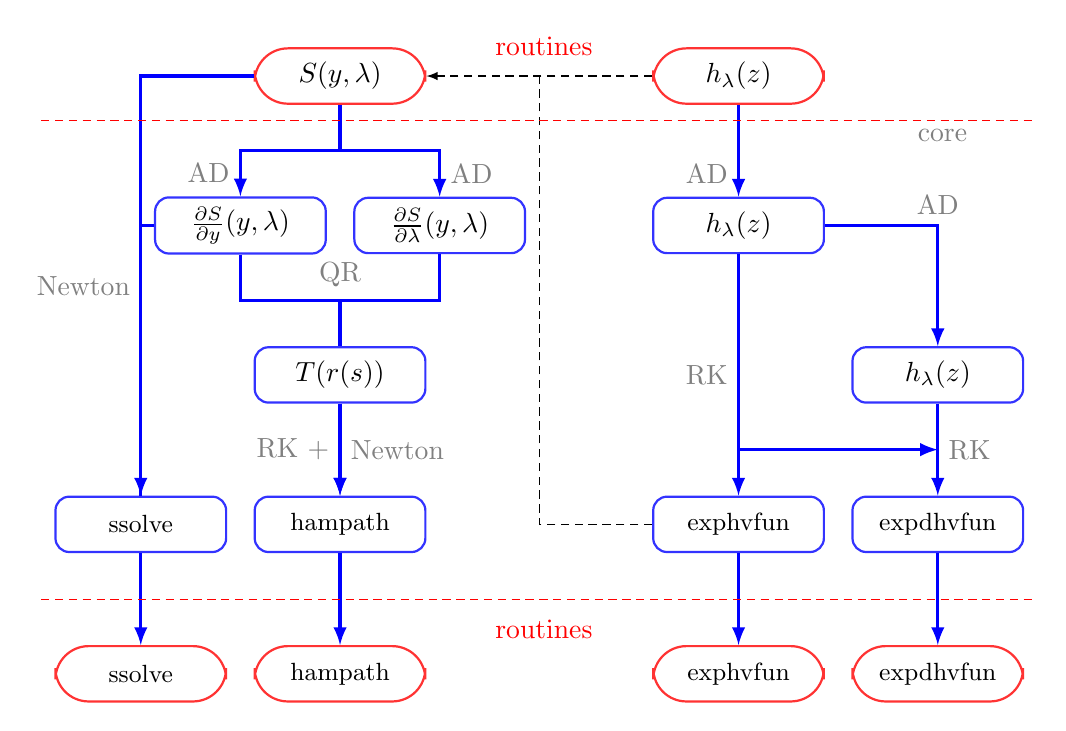
\begin{tikzpicture}[scale=0.9]
            \def\widthBox{5.5em}
%            \tikzstyle{rectcoeur}   =[draw,fill=blue!20,text width=\widthBox,minimum height=2em,text centered,rectangle,rounded corners=5pt]
%            \tikzstyle{rectmat}     =[draw,fill=red!20 ,text width=\widthBox,minimum height=2em,text centered,rectangle,rounded corners=5pt]
%            \tikzstyle{rectfor}     =[draw,fill=red!20 ,text width=\widthBox,minimum height=2em,text centered,rectangle,rounded corners=5pt]
            \tikzstyle{rectcoeur}   =[draw=blue!80, thick, fill=white,text width=\widthBox,minimum height=2em,text centered,rectangle,rounded corners=5pt]
            \tikzstyle{rectmat}     =[draw=red!80 , thick, fill=white,text width=\widthBox,minimum height=2em,text centered,rectangle,rounded corners=12pt]
            \tikzstyle{rectfor}     =[draw=red!80 , thick, fill=white,text width=\widthBox,minimum height=2em,text centered,rectangle,rounded corners=12pt]

            \coordinate (O) at (0,0);
            \def\xshift{8em}
            \def\yshift{6em}

            \node[rectmat]      (B1)    at  (                                           O)  {$S(y,\lambda)$};
            \node[rectmat]      (B2)    at  ([xshift= 2.0*\xshift, yshift= 0.0*\yshift] O)  {$h_\lambda(z)$};
            \node[rectcoeur]    (B12)   at  ([xshift=-0.5*\xshift, yshift=-1.0*\yshift] O)  {$\frac{\partial S}{\partial y}(y,\lambda)$};
            \node[rectcoeur]    (B13)   at  ([xshift= 0.5*\xshift, yshift=-1.0*\yshift] O)  {$\frac{\partial S}{\partial \lambda}(y,\lambda)$};
            \node[rectcoeur]    (B14)   at  ([xshift= 0.0*\xshift, yshift=-2.0*\yshift] O)  {$T(r(s))$};
            \node[rectcoeur]    (B15)   at  ([xshift= 0.0*\xshift, yshift=-3.0*\yshift] O)  {\small \cmd{hampath}      \fortran};
            \node[rectcoeur]    (B16)   at  ([xshift=-1.0*\xshift, yshift=-3.0*\yshift] O)  {\small \cmd{ssolve}       \fortran};
            \node[rectcoeur]    (B21)   at  ([xshift= 2.0*\xshift, yshift=-1.0*\yshift] O)  {$\vv{h_\lambda}(z)$};
            \node[rectcoeur]    (B23)   at  ([xshift= 3.0*\xshift, yshift=-2.0*\yshift] O)  {$\diff\vv{h_\lambda}(z)$};
            \node[rectcoeur]    (B22)   at  ([xshift= 2.0*\xshift, yshift=-3.0*\yshift] O)  {\small \cmd{exphvfun}     \fortran}; 
            \node[rectcoeur]    (B24)   at  ([xshift= 3.0*\xshift, yshift=-3.0*\yshift] O)  {\small \cmd{expdhvfun}    \fortran}; 
            \node[rectfor]      (B17)   at  ([xshift=-1.0*\xshift, yshift=-4.0*\yshift] O)  {\small \cmd{ssolve}       \interface};
            \node[rectfor]      (B18)   at  ([xshift= 0.0*\xshift, yshift=-4.0*\yshift] O)  {\small \cmd{hampath}      \interface}; 
            \node[rectfor]      (B25)   at  ([xshift= 2.0*\xshift, yshift=-4.0*\yshift] O)  {\small \cmd{exphvfun}     \interface};
            \node[rectfor]      (B26)   at  ([xshift= 3.0*\xshift, yshift=-4.0*\yshift] O)  {\small \cmd{expdhvfun}    \interface};

            \draw[->,>=latex, densely dashed        ] (B2.west)     -- (                                     B1.east); %hfun vers sfun
            \draw[   >=latex, densely dashed        ] (B22.west)    -| ([xshift= 1.0*\xshift, yshift= 0.0*\yshift] O); %exphvfun vers sfun
            \draw[   >=latex,very thick,color=blue  ] (B1.south)    -- ([xshift= 0.0*\xshift, yshift=-0.5*\yshift] O); %sfun vers un peu plus bas
            \draw[->,>=latex,very thick,color=blue  ] ([xshift= 0.0*\xshift, yshift=-0.5*\yshift] O) -|   (B12.north)  node[gray,near end,left ] {AD};
            \draw[->,>=latex,very thick,color=blue  ] ([xshift= 0.0*\xshift, yshift=-0.5*\yshift] O) -|   (B13.north)  node[gray,near end,right] {AD};
            \draw[->,>=latex,very thick,color=blue  ] (B2.south)    --                                    (B21.north)  node[gray,near end,left ] {AD};
            \draw[->,>=latex,very thick,color=blue  ] (B21.east)    -|                                    (B23.north)  node[gray,midway  ,above] {AD};
            \draw[->,>=latex,very thick,color=blue  ] (B21.south)   --                                    (B22.north)  node[gray,midway  ,left ] {RK};
            \draw[->,>=latex,very thick,color=blue  ] (B23.south)   --                                    (B24.north)  node[gray,midway  ,right] {RK};
            \draw[->,>=latex,very thick,color=blue  ] (B21.south)   |- ([xshift= 3.0*\xshift, yshift=-2.5*\yshift] O);
            \draw[->,>=latex,very thick,color=blue  ] (B1.west)     -|                                    (B16.north)  node[gray,near end,left ] {Newton};
            \draw[   >=latex,very thick,color=blue  ] (B12.west)    -|                                    (B16.north);
            \draw[->,>=latex,very thick,color=blue  ] (B14.south)   --                                    (B15.north)  node[gray,midway  ,left ] {RK +};
            \draw[->,>=latex,very thick,color=blue  ] (B14.south)   --                                    (B15.north)  node[gray,midway  ,right ] {Newton};
            \draw[->,>=latex,very thick,color=blue  ] (B15.south)   --                                    (B18.north);
            \draw[->,>=latex,very thick,color=blue  ] (B16.south)   --                                    (B17.north);
            \draw[->,>=latex,very thick,color=blue  ] (B22.south)   --                                    (B25.north);
            \draw[->,>=latex,very thick,color=blue  ] (B24.south)   --                                    (B26.north);
            \draw[   >=latex,very thick,color=blue  ] (B12.south)   |- ([xshift= 0.0*\xshift, yshift=-1.5*\yshift] O);
            \draw[   >=latex,very thick,color=blue  ] (B13.south)   |- ([xshift= 0.0*\xshift, yshift=-1.5*\yshift] O);
            \draw[   >=latex,very thick,color=blue  ] ([xshift= 0.0*\xshift, yshift=-1.5*\yshift] O) -- (B14.north) node[gray,above,near start,yshift=0.5em]{QR};

            \draw[densely dashed, color=red         ] ([xshift=-1.5*\xshift, yshift=-0.3*\yshift] O) -- ([xshift= 3.5*\xshift, yshift=-0.3*\yshift] O);
            \draw[densely dashed, color=red         ] ([xshift=-1.5*\xshift, yshift=-3.5*\yshift] O) -- ([xshift= 3.5*\xshift, yshift=-3.5*\yshift] O);

            \node[red]  at ([xshift= 1.0*\xshift, yshift= 0.2*\yshift] O) {\fortran\ routines};
            \node[gray] at ([xshift= 3.0*\xshift, yshift=-0.4*\yshift] O) {\fortran\ core};
            \node[red]  at ([xshift= 1.0*\xshift, yshift=-3.7*\yshift] O) {\interface\ routines};
        \end{tikzpicture}
    \caption{
        Sch\'ema g\'en\'eral de \hampath.
        AD signifie Diff\'erentiation Automatique, RK signifie sch\'emas d'int\'egration num\'erique de Runge-Kutta
        utilis\'es pour la r\'esolution d'\'equations diff\'erentielles ordinaires. L'appellation Newton est employ\'ee
        d\`es qu'un solveur d'\'equations non lin\'eaires de type Newton est appel\'e et enfin QR veut dire factorisation QR.
    }
    \label{fig:schema}
    \end{figure}


%---------------------------------------------------------------------------------------------------------
%---------------------------------------------------------------------------------------------------------


%---------------------------------------------------------------------------------------------------------
%---------------------------------------------------------------------------------------------------------
\section{R\'esolution num\'erique}

\begin{myremark} Se rendre dans le r\'epertoire \cmd{TP\_MI} et ex\'ecuter la commande (dans un terminal) :
    \begin{center}
        \cmd{source hampath\_on}
    \end{center}
    Cette commande doit \^etre ex\'ecut\'ee \`a chaque ouverture d'un nouveau terminal.
\end{myremark}

%------------------------------------------------
\subsection{Probl\`eme \eqref{eq:ocpSimple}}

\begin{myExercice} Se rendre dans le r\'epertoire \cmd{TP\_1\_tir\_simple\_pb\_scalaire/exo\_1}.
    \begin{enumerate}
        \item Jeter un \oe il \`a la routine \cmd{control} du fichier \cmd{afun.f90} codant le contr\^ole $u_s(x,p,p^0) = -p/p^0$, $p^0=-1$.
        \item Jeter un \oe il \`a la routine \cmd{hfun} de \cmd{hfun.f90} codant le hamiltonien maximis\'e 
            $h(z) \coloneqq H(z, p^0, u_s(z, p^0))$, $p^0=-1$, $z\coloneqq (x,p)$ et $H(z,p^0,u) = p(-x+u)+p^0 u^2/2$.
        \item Jeter un \oe il \`a la routine \cmd{sfun} de \cmd{sfun.f90} codant la fonction de tir \eqref{eq:fonctionDeTirSimple}.
            On remarquera l'utilisation de la routine \fortran\ \cmd{exphv} pour l'int\'egration num\'erique du syst\`eme hamiltonien.
        \item Compiler le probl\`eme : ex\'ecuter la commande \cmd{hampathCIMI} dans un terminal dans le r\'epertoire de d\'efinition du probl\`eme.
        \item Jeter un \oe il au script \matlab\ \cmd{main11.m} puis l'ex\'ecuter. V\'erifier que l'on retrouve bien $\psol_0 = \frac{2}{e^2-1}$.
    \end{enumerate}
\end{myExercice}

\begin{myremark}
    \anoter
    Les param\`etres du probl\`eme sont transmis via le vecteur \cmd{par}, des fonctions \matlab\ vers les routines \fortran.
\end{myremark}

%------------------------------------------------
\subsection{Ajout de contraintes sur le contr\^ole}

On consid\`ere le probl\`eme de contr\^ole \eqref{eq:ocpSimple} o\`u l'on ajoute la contrainte sur le contr\^ole par
$u(t) \in \intervalleff{-u_\mathrm{max}}{u_\mathrm{max}}$, $u_\mathrm{max}\coloneqq 1$. La condition de maximisation nous donne comme loi de contr\^ole~:
\begin{equation*}
    %\tag{\ref{eq:controleOCPSimple}$^*$}
    u(t) = 
    \left\{
        \begin{array}{ll}
            u_s(x(t),p(t),p^0) = -p(t)/p^0   & \text{ si } \abs{p(t)} \le u_\mathrm{max}, \\[0.5em]
            +u_\mathrm{max}         & \text{ si } p(t) > u_\mathrm{max}, \\[0.5em]
            -u_\mathrm{max}         & \text{ si } p(t) < -u_\mathrm{max}.
        \end{array}
    \right.
    %\label{eq:controleOCPSimpleContraint}
\end{equation*}

\begin{myExercice} Se rendre dans le r\'epertoire \cmd{TP\_1\_tir\_simple\_pb\_scalaire/exo\_2\_contraintes\_sur\_u}.
    \begin{enumerate}
        \item D\'ecommenter la partie codant pour l'ajout de la contrainte sur le contr\^ole dans le fichier \cmd{afun.f90}.
            Attention, $u_\mathrm{max}$ est donn\'e dans le vecteur \cmd{par}.
        \item Compiler le probl\`eme.
        \item Jeter un \oe il au script \matlab\ \cmd{main12.m} puis l'ex\'ecuter.
    \end{enumerate}
\end{myExercice}


